% This must be in the first 5 lines to tell arXiv to use pdfLaTeX, which is strongly recommended.
\pdfoutput=1
% In particular, the hyperref package requires pdfLaTeX in order to break URLs across lines.

\documentclass[11pt]{article}

% Remove the "review" option to generate the final version.
\usepackage[]{acl}

% Standard package includes
\usepackage{times}
\usepackage{latexsym}
\usepackage{float}
\usepackage{graphicx}

% For proper rendering and hyphenation of words containing Latin characters (including in bib files)
\usepackage[T1]{fontenc}
% For Vietnamese characters
% \usepackage[T5]{fontenc}
% See https://www.latex-project.org/help/documentation/encguide.pdf for other character sets

% This assumes your files are encoded as UTF8
\usepackage[utf8]{inputenc}

% This is not strictly necessary, and may be commented out,
% but it will improve the layout of the manuscript,
% and will typically save some space.
\usepackage{microtype}

% If the title and author information does not fit in the area allocated, uncomment the following
%
%\setlength\titlebox{<dim>}
%
% and set <dim> to something 5cm or larger.

\title{Finding ARG1 of Partitive Nouns in NomBank with DistilBERT}

% Author information can be set in various styles:
% For several authors from the same institution:
% \author{Author 1 \and ... \and Author n \\
%         Address line \\ ... \\ Address line}
% if the names do not fit well on one line use
%         Author 1 \\ {\bf Author 2} \\ ... \\ {\bf Author n} \\
% For authors from different institutions:
% \author{Author 1 \\ Address line \\  ... \\ Address line
%         \And  ... \And
%         Author n \\ Address line \\ ... \\ Address line}
% To start a seperate ``row'' of authors use \AND, as in
% \author{Author 1 \\ Address line \\  ... \\ Address line
%         \AND
%         Author 2 \\ Address line \\ ... \\ Address line \And
%         Author 3 \\ Address line \\ ... \\ Address line}

\author{Ziyang Zeng \\
  Dept. of Computer Science \\
  New York University \\
  251 Mercer Street, New York, NY \\
  \texttt{zz2960@nyu.edu}}

\begin{document}
\maketitle
\begin{abstract}
  This paper presents our attempts of multiple pipelines to find ARG1 of partitive nouns in NomBank with DistilBERT. NomBank is an annotation project at New York University based on Penn Treebank II corpus. Finding ARG1 of partitive nouns in the databank is an semantic role labeling (SRL) problem, which here we treated as a token classification task or a question-answering task. We adopted a knowledge-distilled version of BERT, DistilBERT, into our SRL pipeline, leveraging the knowledge of English Wikipedia and Toronto Book Corpus that the model was originally trained on. For the \% dataset, we achieved an F1 score of 0.9267 on the test set. And for the partitive dataset, we achieved an F1 score of 0.7945 on the test set.
\end{abstract}

\section{Introduction}

NomBank (Meyers et al., 2004c) is a databank project at New York University that adds annotation layer of argument structure for instances in the Penn Treebank II corpus. Apart from the more commonly researched nominalizations of verbs and nominalizations of adjectives, it also covers relational nouns, partitive nouns and several other types of argument-taking nouns.

More recently, the NLP community has seen huge popularity in heavily adopting pretraining-based langauge models in attempt to transfer knowledge learned from large corpus into more specific tasks. BERT (Devlin et al., 2018) is a large-size language representation model trained on a large corpus of English text that can achieve state-of-the-art results on a variety of natural language processing tasks. BERT came a decade later than the release of NomBank and there's been little previous work using it to conduct NomBank-based tasks and related experiments. However, as powerful as BERT is, its large parameters size makes it significantly more computationally expensive to train and use. On the other hand, DistilBERT is a distilled student model of BERT that retains 97\% of BERT's language understanding capabilities while being 40\% smaller and 60\% faster. This makes it a great candidate to train when facing with limited resources.

This paper presents multiple token classification approaches using pre-trained DistilBERT to find ARG1 of partitive nouns in NomBank. It focuses on partitive nouns (nouns that are used to describe a part or quantity of something) and the partitive task. The task is described as finding one argument (ARG1) of \% (the percent sign), or in other words, finding the none group that is being sub-divided or quantified over. For example, for the sentence "Output in the energy sector rose 3.8\%.", the ARG1 to be found is "Output" since it is the partitive noun that "3.8\%" is referring to. This task can be translated into a binary classification problem on each token in the sentence where the model predicts whether the token is an ARG1 or not.

In addition to the token classification approaches above, this paper also experiments with question-answer task, transforming the original ARG1 finding task into the task of make the model answer the question "What is the ARG1 of this sentence?". The advantage of this adaptation is that the model would stably output exactly one ARG1 for each sentence whereas token classification could give each sentence 0 to N ARG1s.


\section{Related Work}

NomBank (Meyers et al., 2004c), as a databank extending the frames of NOMLEX and PropBank, annotates argument structures of common nouns similar to how PropBank annotates predicating verbs. The development of the NomBank corpus has made several other work on argument structure extraction more accessible. Jiang and Ng (2006) attempts the first NomBank-based automatic semantic role labeling system after the databank's release. Ping (2006)  adapts a PropBank-based SRL system to the SRL task of NomBank, achieving an overall F1 score of 72.73 on section 23 of the NomBank corpus.

BERT, or Bidirectional Encoder Representations from Transformers (Devlin et al., 2018), has shown state-of-the-art results on many NLP tasks. The BERT base model has 110 million trainable parameters and was trained on a concentration of English Wikipedia and Toronto Book Corpus. There have been many attempts to compress BERT into a smaller model, among which DistilBERT (Sanh et al., 2019) successfully reduces the size of a BERT model by 40\%, while retaining 97\% of its language understanding capabilities and being 60\% faster, leveraging  knowledge distillation (Bucila et al., 2006, Hinton et al., 2015) during the pre-training phase.

More recent development on semantic role labeling (SRL) has shifted from feature engineering to architecture-based modeling leveraging deep neural networks (Collobert
et al., 2011). Several recent notable approaches suggest only using raw tokenized text as input and let the model learn the features from the text itself (He et al., 2017; Sahin and Steedman, 2018; Marcheggiani et al., 2017; Strubell et al., 2018). This end-to-end approach allows the model to easily generalize from one SRL task to another without very task-specific feature engineering effort.

\section{ARG1 Finding Pipelines}

\subsection{Maximum Entropy Baseline Pipeline}

The baseline we use is a maximum entropy machine learning method in a token-by-token classification manner. Maximum entropy is a general technique for estimating probability distributions from data. Labeled training data
is used to derive a set of constraints for the model that
characterize the class-specific expectations for the distribution. To perform well, the model relies on the good representation of the features we feed it. In this paper, we select features including the word stem, the neighboring 2 words, POS tags, NG-BIO tags, whether capitalized and the position of the word in the sentence. Figure \ref{fig:maxent-feature-sample} shows the features we selected for the maximum entropy baseline.

\begin{figure}[h]
  \centering
  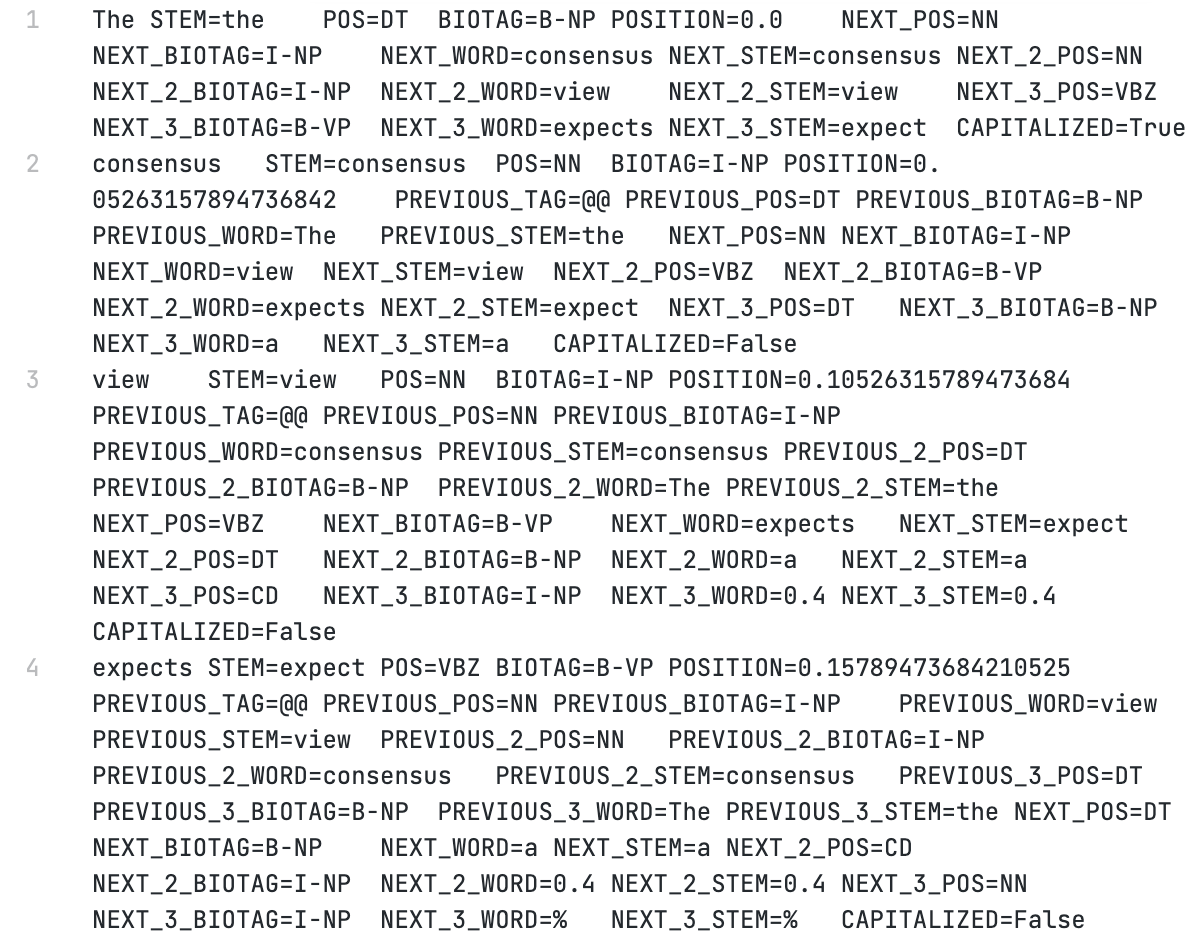
\includegraphics[width=\linewidth]{assets/maxent-feature-sample.png}
  \caption{Sample sentence features for maxent system}
  \label{fig:maxent-feature-sample}
\end{figure}

\subsection{Plain Raw Input Pipeline}
\label{section:plain-pipeline}

The simplest pipeline for finding ARG1 of partitive nouns in NomBank assumes that the input text is raw and unprocessed. The pipeline first tokenizes the text using the tokenizer provided by DistilBERT. Then, the model predicts whether each token is an ARG1 or not. The pipeline is illustrated in the following figure \ref{fig:simplest-arg1-pipeline}.

However, the NomBank dataset provisions text as already tokenized. The way the tokenizer provided by DistilBERT is often more fine-grained than how the NomBank dataset provides the text, causing some aligning issues. We fix this by align the tokens using \verb|word_ids| in the tokenization output. This is explained in detailed in section \ref{section:data-preprocessing}.

\begin{figure}[h]
  \centering
  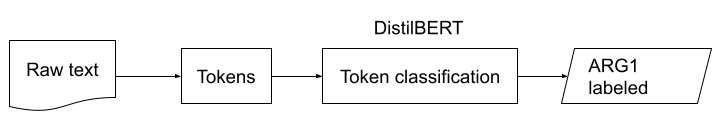
\includegraphics[width=\linewidth]{assets/simplest-arg1-pipeline.png}
  \caption{The simplest pipeline for finding ARG1 of partitive nouns in NomBank}
  \label{fig:simplest-arg1-pipeline}
\end{figure}

In practice, this pipeline has the tendency of over predicting ARG1 labels. It predicts on a per-token basis, making classification of whether the token is an ARG1 or not on every token, thus possibly producing 0 to multiple ARG1s in one sentence. It is shown by our experiments that the deep models are more common to produce more than 1 ARG1s in one sentence. The ground truth, however, is one and only one ARG1 per sentence. A treatment of this inconsistency is to always force one ARG1 by the logits output of the deep neural network. We assign the token with the largest logit value in the output vector for the whole sentence to be the ARG1.

\subsection{Feature Enhanced Pipeline}

NomBank provides a number of features for each token in the databank, including POS tags and NG-BIO tags. They could be helpful for the task of finding ARG1 of partitive nouns. The pipeline below incorporate these features to the raw text input in \ref{section:plain-pipeline} to find ARG1 of partitive nouns. The pipeline is illustrated in the figure \ref{fig:enhanced-arg1-pipeline}.

\begin{figure}[h]
  \centering
  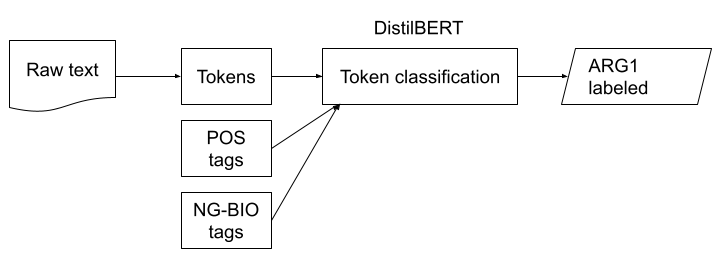
\includegraphics[width=\linewidth]{assets/enhanced-arg1-pipeline.png}
  \caption{The feature-enhanced pipeline for finding ARG1 of partitive nouns in NomBank}
  \label{fig:enhanced-arg1-pipeline}
\end{figure}

Because the original pre-trained DistilBERT model does not take extra features including POS and NG-BIO tags as input, we have to modified the token classification model and alter the last linear layer, concatenating the original BERT hidden layer output with the extra features, then doing token classification through the linear layer.

\subsection{Question-Answer Pipeline}

Apart from token classification, we also explored question-answer approach which rephrase the original problem into a QA problem. Question-answering, just as the plain token classification approach, assumes tokenized input and no extra features. Additionally, question-answering tasks also requires a question prompt and answer location for each sample while training. The pipeline is illustrated in the figure \ref{fig:qa-arg1-pipeline}.

\begin{figure}[h]
  \centering
  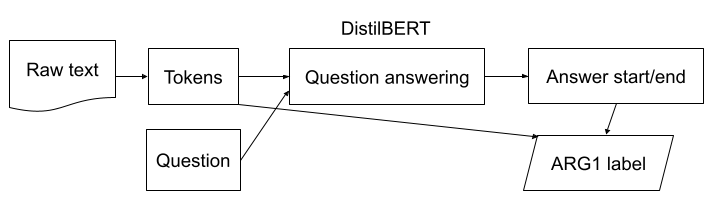
\includegraphics[width=\linewidth]{assets/qa-arg1-pipeline.png}
  \caption{The question-answering pipeline for finding ARG1 of partitive nouns in NomBank}
  \label{fig:qa-arg1-pipeline}
\end{figure}

The output of the question-answering model is the location (start index and end index) of the predicted answer. By locating the token on the original input token list with the start index and end index, we can reconstruct the ARG1 label of the sentence. The answer relocation is a bit more complicated due to the tokenization discrepancies between the original input and the tokenized input. Again, this is explained in detailed in section \ref{section:data-preprocessing}.

\section{Experiments}

\subsection{Dataset}

The dataset we use in this task is part of the NomBank that specifically focus on partitive nouns. In the dataset is split into training, dev and test set. The training set has 2367 sentences or 66186 words, the dev set has 83 sentences or 2225 words, and the test set has 150 sentences or 4276 words. Each token in a sentence takes a line in the data file, the line containing the token itself, the POS tag, the NG-BIO tag, the index of the sentence and the index of the token in the sentence. The semantic role label is put at the end of each line, if the label is not one of "ARG1", "PRED" and "SUPPORT", then it's omitted. Figure \ref{fig:dataset-one-sample} is one sample sentence from the training dataset.

\begin{figure}[h]
  \centering
  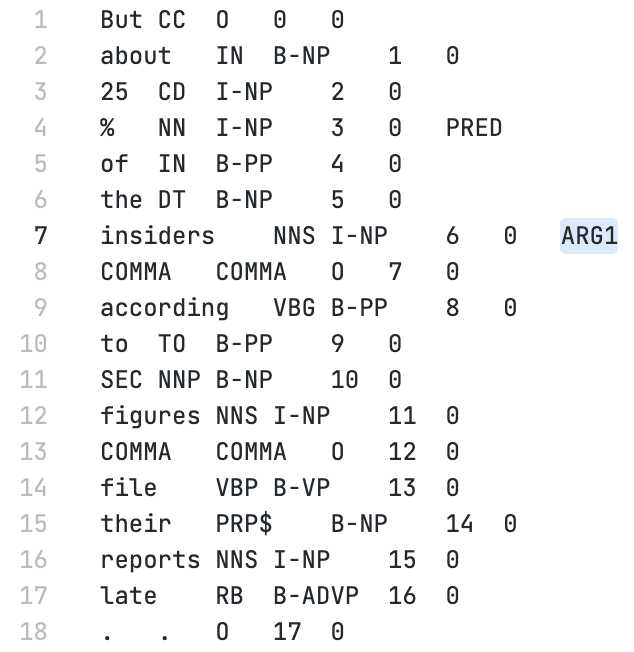
\includegraphics[width=\linewidth]{assets/dataset-one-sample.png}
  \caption{One sample sentence in the training dataset}
  \label{fig:dataset-one-sample}
\end{figure}

In a sentence in the \% dataset, the PRED labels \% symbol, the ARG1 is the partitive noun that \% symbol refers to, and the SUPPORT marks the word connecting the ARG1 and the PRED. It is guaranteed that there is one and only one ARG1 in each sentence of the dataset.

\subsection{Data Preprocessing}
\label{section:data-preprocessing}

Even though for deep neural network input wouldn't need much feature engineering, we still need to tokenize the text and convert the text into numerical representation so that it can be served as the input of the model. For DistilBERT-based pipelines, the tokenizer provided by DistilBERT is used to tokenize the text. However, the dataset is already tokenized and the way DistilBERT tokenizes a sentence could be different from how the sentences are already tokenized in the dataset. More specifically, the tokenizer from DistilBERT could tokenize the sentence into even smaller tokens than the tokenizer used in the dataset. Therefore, this could cause the output label of the model fail to align with the input given. Fortunately, the results of the DistilBERT tokenizer include the align information for the tokenization. With this information, we can reconstruct the tokenized sentence from the DistilBERT tokenizer output and match the model output with the original input.

\begin{figure}[h]
  \centering
  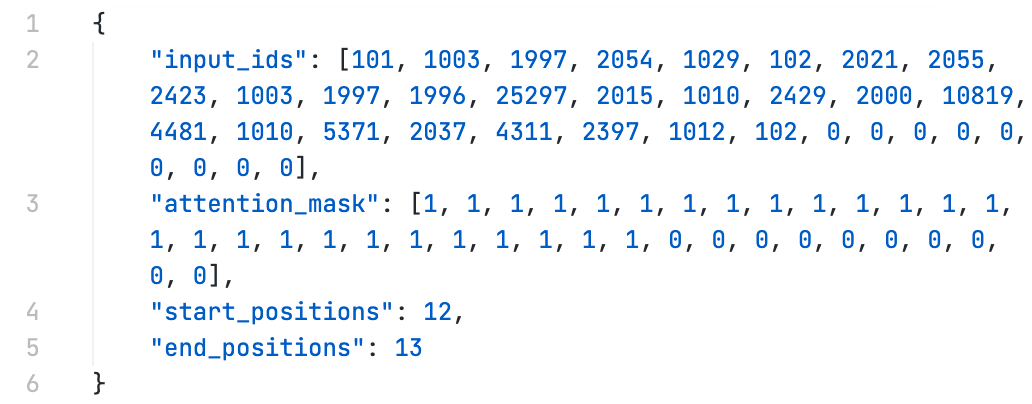
\includegraphics[width=\linewidth]{assets/dataset-one-qa-sample.png}
  \caption{One sample sentence for QA task}
  \label{fig:dataset-one-qa-sample}
\end{figure}

A special treatment for the question-answering pipeline is that the ARG1 label has to be transformed into the answer location (the start and end indexes). And the question prompt for every sample is the same "What is the ARG1 of the sentence?". The exact same question prompt is used for validation and testing. Figure \ref{fig:dataset-one-qa-sample} is one processed sample sentence for the QA task, inputs are padded in batch and stacked as matrix to be able to be processed by the model in batches. \verb|input_ids| are the numerized tokens of both the question prompt and the input text concatenated by \verb|102|. \verb|attention_mask| is the attention the model should be given to the tokens, \verb|0| means the token should not be considered by the model. \verb|start_position| and \verb|end_position| are the start and end indexes of the answer in the input text.


\subsection{Experiment Settings}

All deep models used in this paper are implemented in PyTorch and with HuggingFace transformers libraries. The pre-trained models are fine-tuned on a single NVIDIA P100 (16GB) GPU on the Google Colab platform. The deep models are fine-tuned for 10 epochs with the learning rate of \verb|2e-5| and weight decay of \verb|0.01|. For token classification tasks, the batch size is 64. For question-answering tasks, the input would be bigger with the question prompt, so the batch size is set to 32 to be able to fit into the GPU's RAM.

\subsection{Evaluation Metrics}

To evaluate the performance of the model, we used precision, recall and F1-score as evaluation metrics. The precision and recall are calculated by the number of correct predictions divided by the total number of predictions. The F1-score is calculated by the harmonic mean of precision and recall. Below are the formulas for calculating the precision, recall and F1-score, in which TP is the number of true positives, FP is the number of false positives, FP is the number of false positives and FN is the number of false negatives.

\begin{equation}
  Precision={TP\over{TP+FP}}
\end{equation}

\begin{equation}
  Recall={TP\over{TP+FN}}
\end{equation}

\begin{equation}
  F1={2\times{Precision}\times{Recall}\over{Precision+Recall}}
\end{equation}

\subsection{Partitive Dataset}

Apart from the original \% task, we also experimented the token classification of DistilBERT on the combined dataset of \% and partitive datasets of NomBank. Different from the \% dataset, there's not only ARG1 but also ARG0, ARG2... and more role labels in the partitive dataset. In order to adopt the same pipelines, we preprocessed the partitive dataset into the same format as the \% dataset and combine them together into a larger dataset. The larger dataset is also split into training, dev and test set. The training set has 12991 sentences or 380247 words, the dev set has 426 sentences or 12671 words, and the test set has 746 sentences or 21536 words.

The partitive dataset, in comparison with the \% dataset, has more distractions in terms of ARG1 finding task since ARG0, ARG2 and other labels are given. Also, there could be more than one or zero ARG1s in one sentence, thus making our QA and ONE ARG1 pipelines useless since the tendency of producing only one ARG1 is no longer preferred.

\section{Experiment Results}

\begin{table*}
  \centering
  \begin{tabular}{c||c|c|c}
    \hline
    \textbf{Model}        & \textbf{Precision} & \textbf{Recall} & \textbf{F1-Score} \\
    \hline
    MaxEnt Baseline       & {71.88\%}          & {61.33\%}       & {66.19\%}         \\
    DistilBERT            & {93.75\%}          & {90.00\%}       & {91.84\%}         \\
    DistilBERT (POS+BIO)  & {93.19\%}          & {91.33\%}       & {92.25\%}         \\
    DistilBERT (QA)       & {92.00\%}          & {92.00\%}       & {92.00\%}         \\
    DistilBERT (ONE ARG1) & {92.67\%}          & {92.67\%}       & {92.67\%}         \\
    \hline
  \end{tabular}
  \caption{Precision, Recall and F1-Score on the \% dataset}
  \label{tab:results-on-first-dataset}
\end{table*}

\begin{table*}
  \centering
  \begin{tabular}{c||c|c|c}
    \hline
    \textbf{Model}       & \textbf{Precision} & \textbf{Recall} & \textbf{F1-Score} \\
    \hline
    MaxEnt Baseline      & {55.33\%}          & {36.02\%}       & {43.64\%}         \\
    DistilBERT           & {80.49\%}          & {78.43\%}       & {79.45\%}         \\
    DistilBERT (POS+BIO) & {81.53\%}          & {76.94\%}       & {79.16\%}         \\
    \hline
  \end{tabular}
  \caption{Precision, Recall and F1-Score on the partitive dataset}
  \label{tab:results-on-partitive-dataset}
\end{table*}

We experimented with multiple ARG1 finding models and pipelines on both \% dataset and partitive dataset from the NomBank corpus. The results are shown in Table \ref{tab:results-on-first-dataset} and Table \ref{tab:results-on-partitive-dataset} respectively.

For the partitive dataset, because there could be zero or multiple ARG1s in one sentence for ground truth, there's no need to force model to predict only one ARG1, thus we abandoned the QA and ONE ARG1 pipelines for the partitive dataset.

As shown by Table \ref{tab:results-on-first-dataset}, the MaxEnt baseline achieved an F1 score of \verb|0.6619|. The DistilBERT models perform much better than the MaxEnt Baseline model on the \% dataset generally even when given less features, achieving an F1 score of 0.9184 for the basic pipeline,  \verb|0.9225| for the feature-enhanced pipeline,  \verb|0.92| for the QA pipeline and  \verb|0.9267| for the ONE ARG1 pipeline. The performance differences between different DistilBERT-based pipelines, however, are not significant. POS tags and NG-BIO tags likely don't have much effect on the performance of the model.

As for the partitive dataset, it is also shown by Table \ref{tab:results-on-partitive-dataset} that the DistilBERT model performs better than the MaxEnt Baseline model that achieved an F1 score of  \verb|0.4364|. The basic pipeline achieved an F1 score of  \verb|0.7945|. It is also observed that the POS tags and NG-BIO tags features didn't have significant impact on the performance of the model, achieving an F1 score of only  \verb|0.7916|.

\section{Conclusion}

\section{Future Work}

\section*{References}

This document has been adapted
by Steven Bethard, Ryan Cotterell and Rui Yan
from the instructions for earlier ACL and NAACL proceedings, including those for
ACL 2019 by Douwe Kiela and Ivan Vuli\'{c},
NAACL 2019 by Stephanie Lukin and Alla Roskovskaya,
ACL 2018 by Shay Cohen, Kevin Gimpel, and Wei Lu,
NAACL 2018 by Margaret Mitchell and Stephanie Lukin,
Bib\TeX{} suggestions for (NA)ACL 2017/2018 from Jason Eisner,
ACL 2017 by Dan Gildea and Min-Yen Kan,
NAACL 2017 by Margaret Mitchell,
ACL 2012 by Maggie Li and Michael White,
ACL 2010 by Jing-Shin Chang and Philipp Koehn,
ACL 2008 by Johanna D. Moore, Simone Teufel, James Allan, and Sadaoki Furui,
ACL 2005 by Hwee Tou Ng and Kemal Oflazer,
ACL 2002 by Eugene Charniak and Dekang Lin,
and earlier ACL and EACL formats written by several people, including
John Chen, Henry S. Thompson and Donald Walker.
Additional elements were taken from the formatting instructions of the \emph{International Joint Conference on Artificial Intelligence} and the \emph{Conference on Computer Vision and Pattern Recognition}.

% Entries for the entire Anthology, followed by custom entries
\bibliography{anthology,custom}
\bibliographystyle{acl_natbib}

\end{document}
